
\chapter{基于多帧散斑照明的散射介质3D目标成像}

在前面章节中,我们对基于OME卷积成像模型进行了介绍,通过数值仿真和实验验证的方式,对散斑自相关的基本成像原理进行研究,研究了不同相位恢复算法的特点实现透过散射介质彩色成像和基于散斑的之间相的关性提出新型的非入侵透过散射介质成像方法。在第\ref{chap:5}章节中,我们所提出的方法能够有效的恢复超出光学记忆的目标,实现了对于扩展目标的非入侵成像。然后,如何有效的实现透过散射介质3D成像仍具有挑战性,以上的方法都具有各自的局限性,无法有效地解决透过散射介质的3D成像。

\begin{figure}[htp]
	\centering
	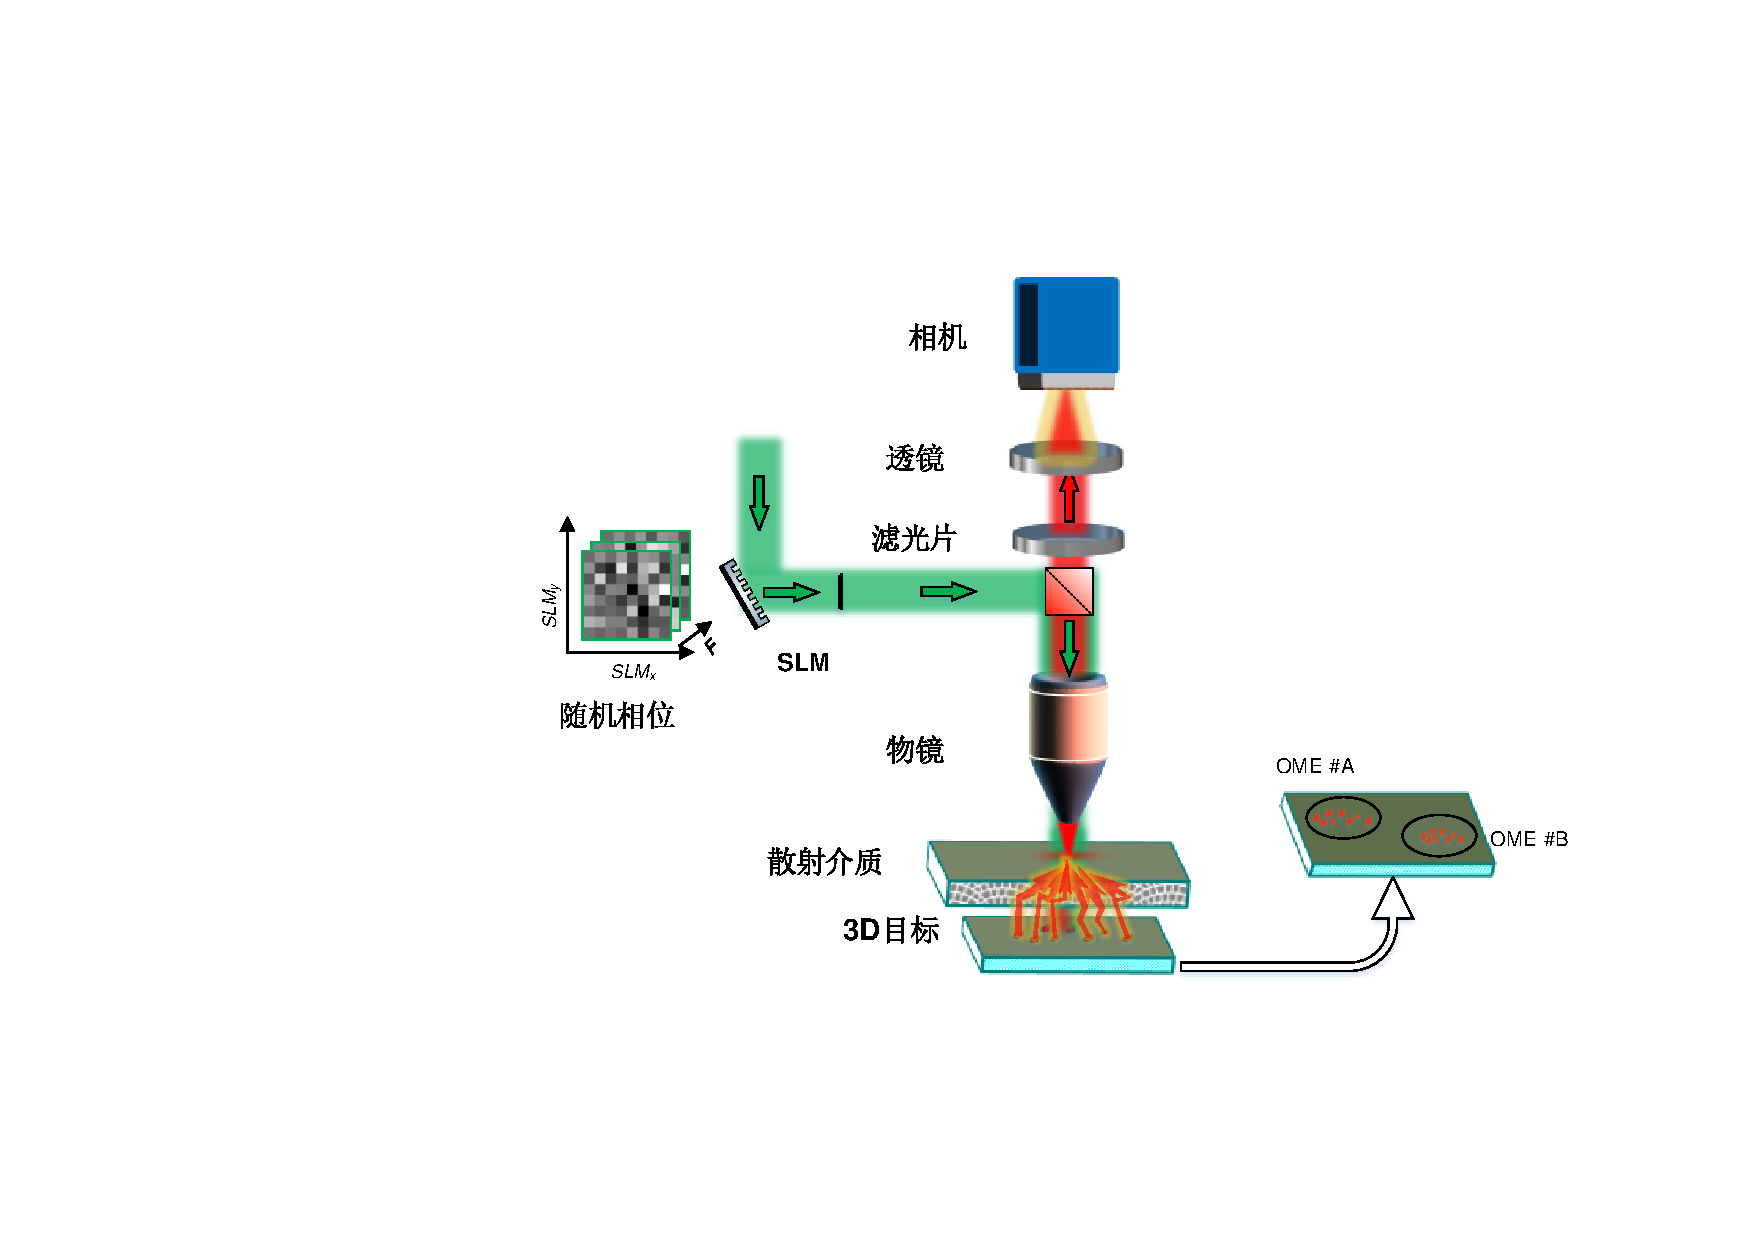
\includegraphics[scale=0.75]{C6.fig1}
	\caption{多帧散斑照明的散射3D目标成像示意图}
	\label{fig:6.1}
\end{figure}

针对透过散射介质进行3D目标成像问题已经进行多年,目前已有的方法可以大致分为以下三个方面:第一,利用散射介质的空间去相关特性,对系统的PSF进行预标定,实现不同景深或者不同视场的图像拼接;第二,利用参考目标或者放置点源目标的方式,然后从复杂信号中提取目标信息并进行图像重建;第三,测量光学传输矩阵,获得更大范围光场的控制,进而实现大视场扫描成像。利用散射介质的先验信息、放置参考目标的方式或者测量光学传输矩阵方法,虽然在一定程度上实现了透过散射介质的大视场或者3D目标成像,但是难以在非入侵的条件下进行实施。与第\ref{chap:5}章节中所展示的结果不同,本章我们重点研究当空间存在多个目标,不同的目标位于不同OME范围,如何进行有效地进行图像重建。受到第\ref{chap:5}章节方法的启发,我们可以通过随机照明的方式,获得系统中不同点光源的散斑指纹,但是当有效的获取散斑指纹后该如何进行重建将在接下来部分进行讨论。同时受到机器学习、图像分类和模式识别相关工作的启发,我们提出了一种非入侵透过散射介质3D目标成像方法,利用随机照明的方式获得散斑图案进行去混叠获得散斑指纹,对散斑指纹进行分类,并最终实现了透过散射介质的3D成像。我们的方法特点在于:(\romannum{1})只需散斑照明;(\romannum{2})无需相位恢复;(\romannum{3})与散斑自相关成像方法相比,能够更好的重建图像,具有较高的图像分辨率。

由于目前针对于散射成像的研究方向更倾向于与生物成像像交叉的方法,同时荧光成像方式在生物成像方面有着更多的应用,因此本章所描述的成像方法及成像构架均以荧光目标成像为章节主线。然后,我们所提出的方法同样能够扩展至拉曼和多光子成像等领域。

\section{基于多帧散斑照明的散射介质3D目标成像基本原理}

\subsection{3D目标成像模型}

成像系统如图\ref{fig:6.1}所示,当激光通过SLM时,入射激光被添加了随机相位实现调制,进而利用随机散斑照明目标后,目标产生自身的激发光,激发光传播并通过散射介质,产生散斑最终被相机所接收,此时相机所获得的散斑为不同散斑指纹的非相干总和。此外,光学记忆效应范围内的独立点光源将在相机上产生相关但平移的散斑指纹 \cite{Freund1988},而光学记忆效应范围外的点光源将产生完全不相关的散斑指纹。对于给定的散斑照明,捕获的图像 $I_{\textsl{fluo}}$ 可以表示为具有不同权重的散斑指纹的线性叠加。因此,相机图像$I_{\textsl{fluo}}$由下式给出:

\begin{equation}
\begin{aligned}
I_{fluo}(r,t) = \sum^{P}_{k=1} w_{k}(r) h_{k}(t),
\label{eq:6.1}
\end{aligned}
\end{equation}
其中,$I_{fluo}(r,t)$为对应于第$t$次照明时相机所接收到低对比度散斑,$r$为空间坐标,$w_{k}(r)$为第$k$个独立点光源所对应的散斑指纹,$h_{k}(t)$为第$t$次照明时第$k$个独立点光源所接收到的激光光的强度,$P$为系统中独立点光源的数量。

在此成像模型下,假设不同OME范围的PSF已知,图像可以通过简单的去卷积过程进行重建。但是在实际生物成像应用中,获取系散射介质的PSF往往难度较大或者难以实现。受到第\ref{chap:5}章节方法的启发,我们对获得的散斑图像序列利用NMF算法进行去混叠,进而获得不同点光源的散斑指纹。然后,在获得散斑指纹后,如何进行图像重建将是本章的重点。由于去混叠部分与第\ref{chap:5}章节所展示的部分完全相同,所以在此处不进行重复描述。

在此,假设我们的系统中存在目标A和目标B,它们分别位于不同的OEM范围。因此,公式(\ref{eq:6.1})可以写为:
\begin{equation}
\begin{aligned}
I_{fluo}(r,t) = \sum^{P}_{k=1} w_{k}^{A}(r) h_{k}^{A}(t)+\sum^{P}_{k=1} w_{k}^{B}(r) h_{k}^{B}(t),
\label{eq:6.2}
\end{aligned}
\end{equation}
其中,$h_{k}^{A}(t)$和$h_{k}^{B}(t)$分别代表来自目标A和目标B的散斑指纹。假设可以将公式(\ref{eq:6.1})表示为公式(\ref{eq:6.2})的形式,目标A和B分别可以利用第\ref{chap:5}章节所呈现的方法进行重建。

当进行去混叠步骤后,$h_{k}^{A}(t)$和$h_{k}^{B}(t)$被获取,探索不同指纹之间的相关性,将有助于图像重建。受到OME启发,光学记忆效应范围内的独立点光源的散斑指纹之间相关但是之间具有平移\cite{Freund1988},而光学记忆效应范围外的点光源散斑指纹完全不相关。在空间域的位移,在傅里叶域来看的的话,空间的平移对应于频域的斜坡相位,即:
\begin{equation}
\begin{aligned}
\mathcal{F}(h_i^{A}(t)) = \mathcal{F}(h_j^{A}(t))*\mbox{exp}[i\phi_{ramp}]
\label{eq:6.3}
\end{aligned}
\end{equation} 对公式(\ref{eq:6.3})两边同时求绝对值(同傅里叶振幅),即:
\begin{equation}
\begin{aligned}
\mbox{abs} \{ \mathcal{F}(h_i^{A}(t)) \} = \mbox{abs} \{  \mathcal{F}(h_j^{A}(t))*\mbox{exp}[i\phi_{ramp}] \}
\label{eq:6.4}
\end{aligned}
\end{equation}其中,$\mbox{abs}$表示求绝对值运算。

从公式(\ref{eq:6.4})可知,位于同一OME范围内的点光源所对应的散斑指纹的傅里叶变换后,它们的傅里叶振幅接近相等,相关仿真结果如图\ref{fig:6.2}所示。图\ref{fig:6.2}中,(a)和(b)为位于同一OME范围内,不同点光源的散斑指纹;(c)和(d)分别为散斑(a)和(b)的傅里叶变换后的振幅显示;(e)为(c)和(d)图中心切线的强度曲线;(f)和(g)为位于同一OME范围内,不同点光源的散斑指纹;(h)和(i)分别为散斑(f)和(g)的傅里叶变换后的振幅显示;(j)为(h)和(i)图中中心切线的强度曲线;图(k)为图(c)、(d)、(h)和(i)中心切线的强度分布图。由图\ref{fig:6.2}(k)所显示的结果可知,曲线一和曲线二非常接近,曲线三和曲线四非常接近,曲线一、二和曲线三、四之间的差异较大,此结果证明了上部分的理论推导。

同OME范围的散斑在傅里叶域的傅里叶振幅信息极其接近,不同OME范围的散斑在傅里叶域的傅里叶振幅信息差异较大,此信息在后续的部分将被用来作为散斑分类的判定准则。但是,如何巧妙地设计散斑分类方法,也是问题的难点之一。在接下来的散斑分类中,我们将利用多位缩放(Multidimensional Scaling,MDS)算法进行散斑分类,该方法在机器视觉和数据图形化领域应用较为广泛。
\begin{figure}[htp]
	\centering
	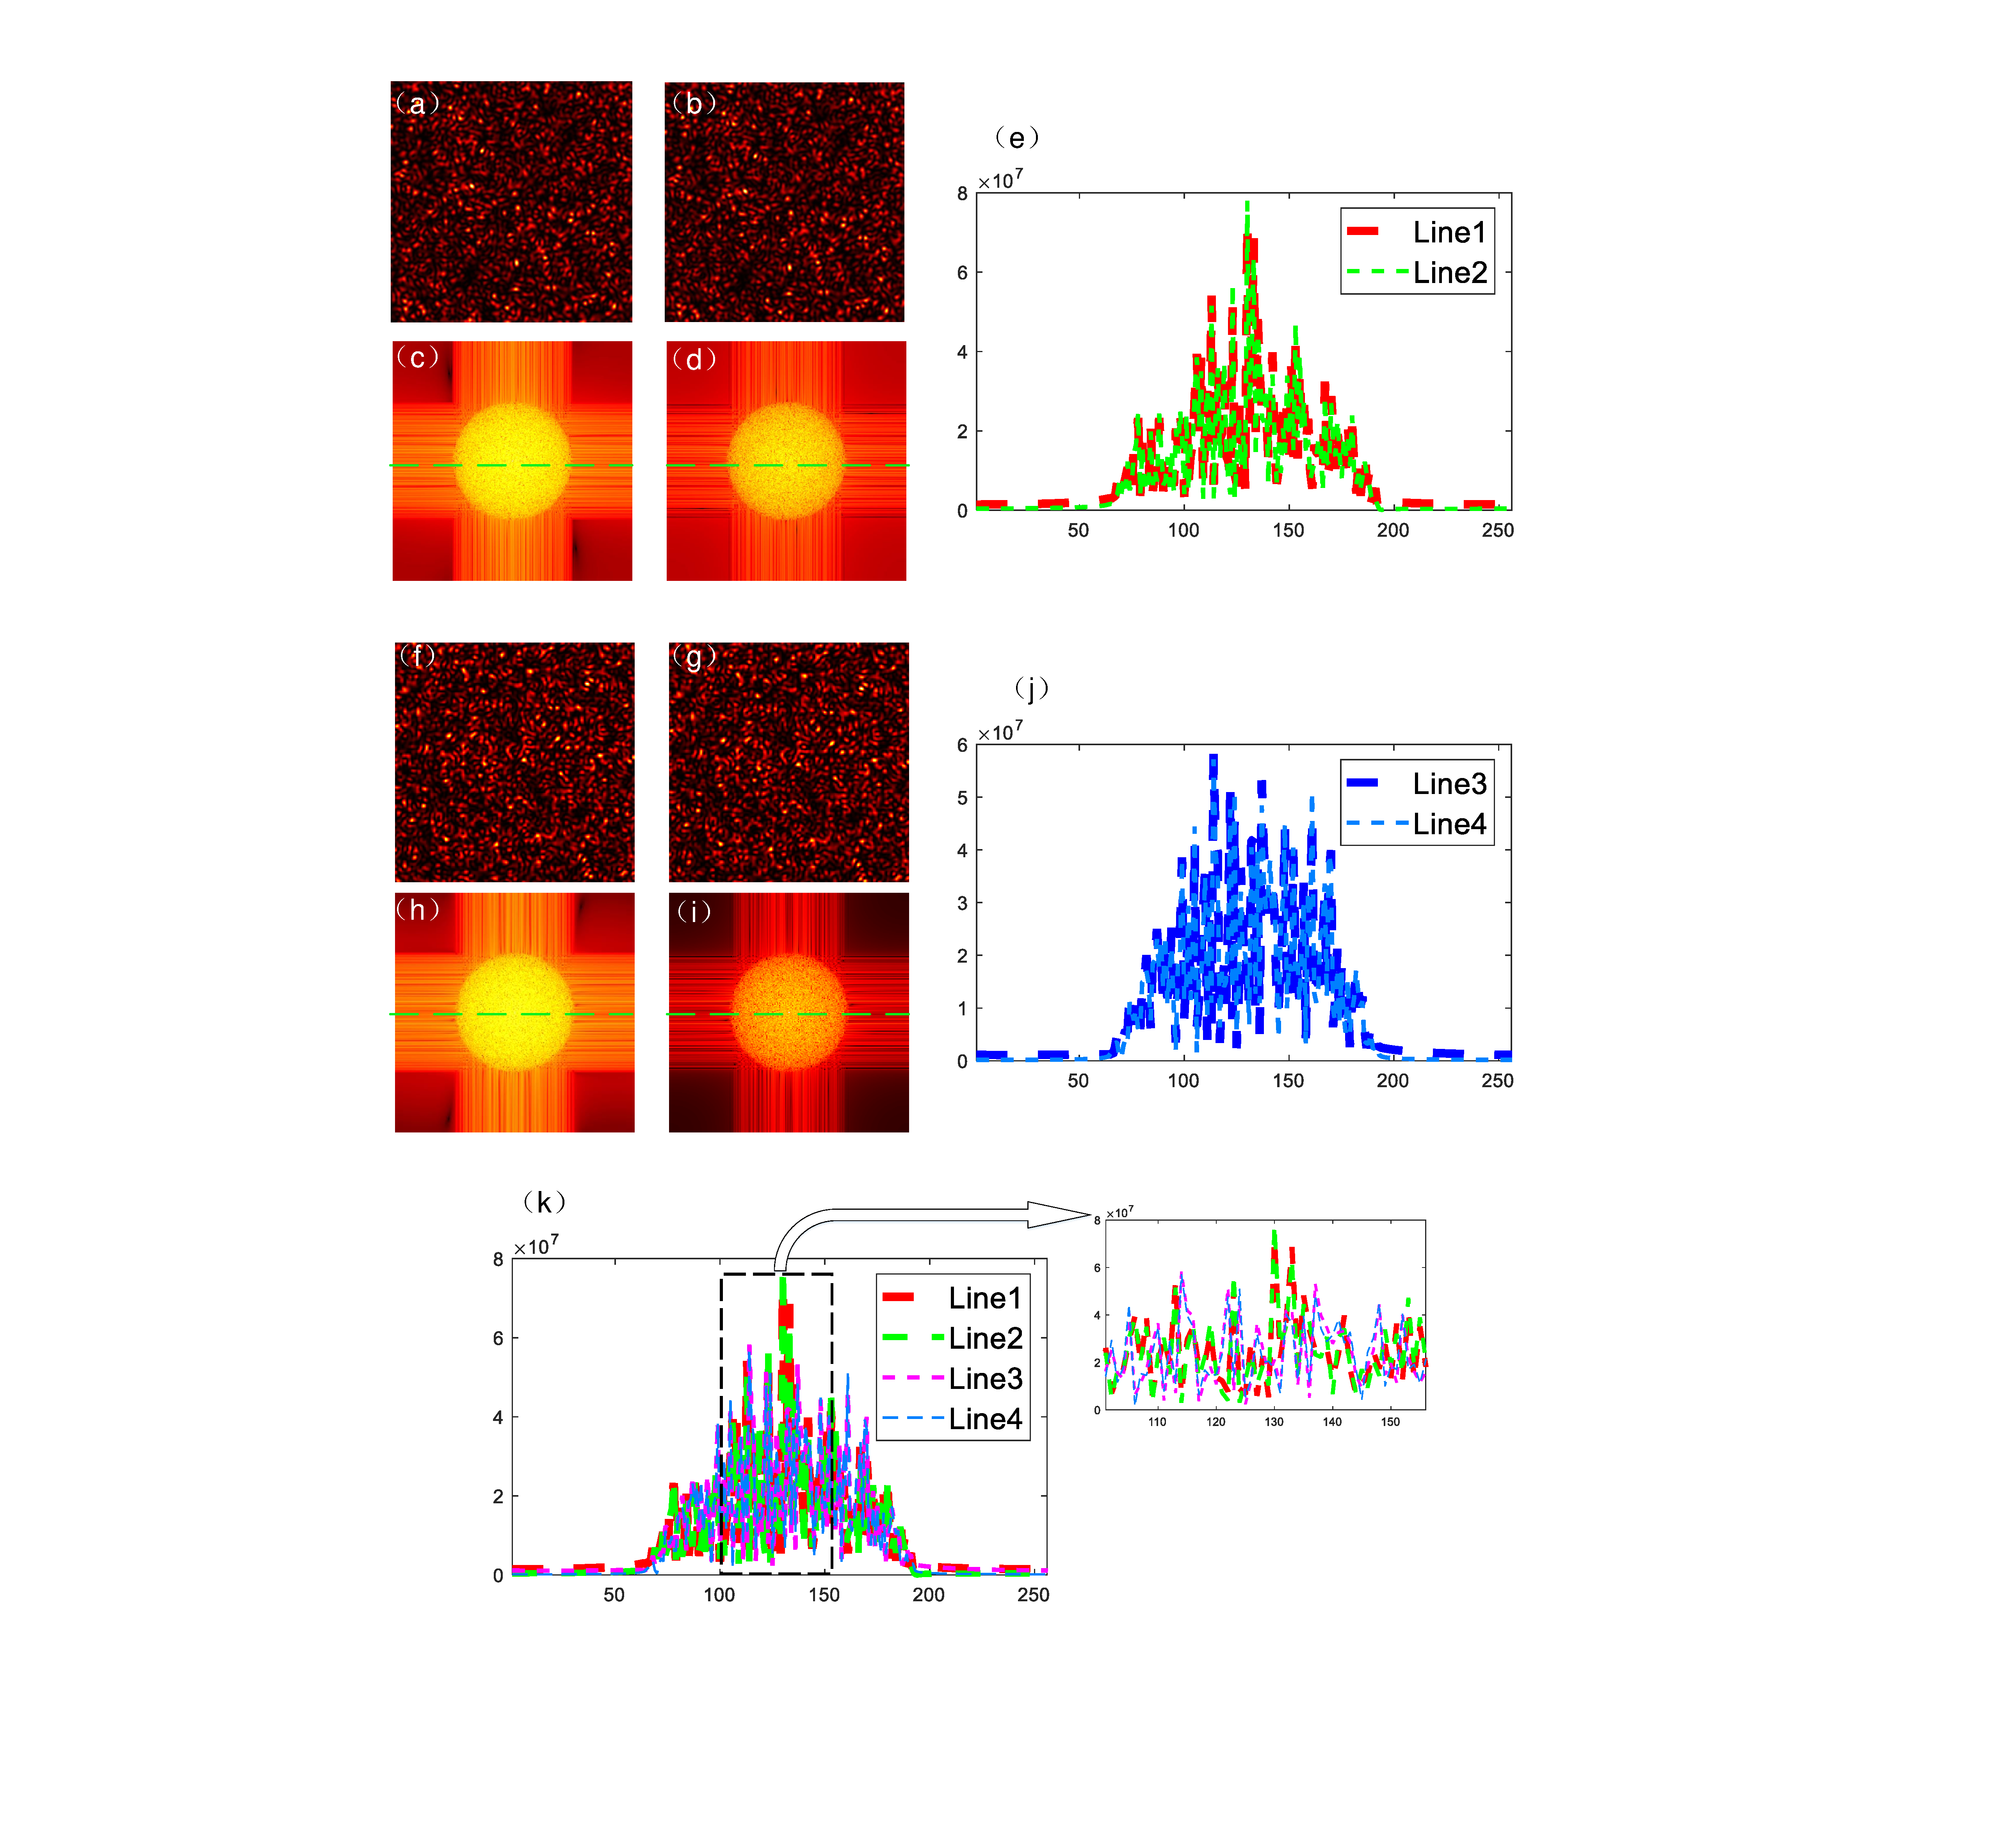
\includegraphics[scale=0.30]{C6.fig2}
	\caption{不同OME范围散斑指纹之间傅里叶振幅信息探索}
	\label{fig:6.2}
\end{figure}

\subsection{3D目标重建过程}
